\chapter{Evaluation\label{cha:evaluation}}

In this chapter the Orchestrator introduced in chapter \ref{cha:orchestrator} is tested and evaluated. For this purpose an object detection application is used, which should be deployed to a given test infrastructure containing several devices. In the first experiment the nodes join and leave the network one after the other. In the second experiment all nodes are online, but the network connection quality is manipulated. For both experiments it is examined which decisions the Orchestrator takes and what effect this decision has on the total latency of the application.

\section{Experimental setup}

\subsection{Infrastructure\label{sec:eval-infrastructure}}

\begin{figure}[htb]
    \centering
    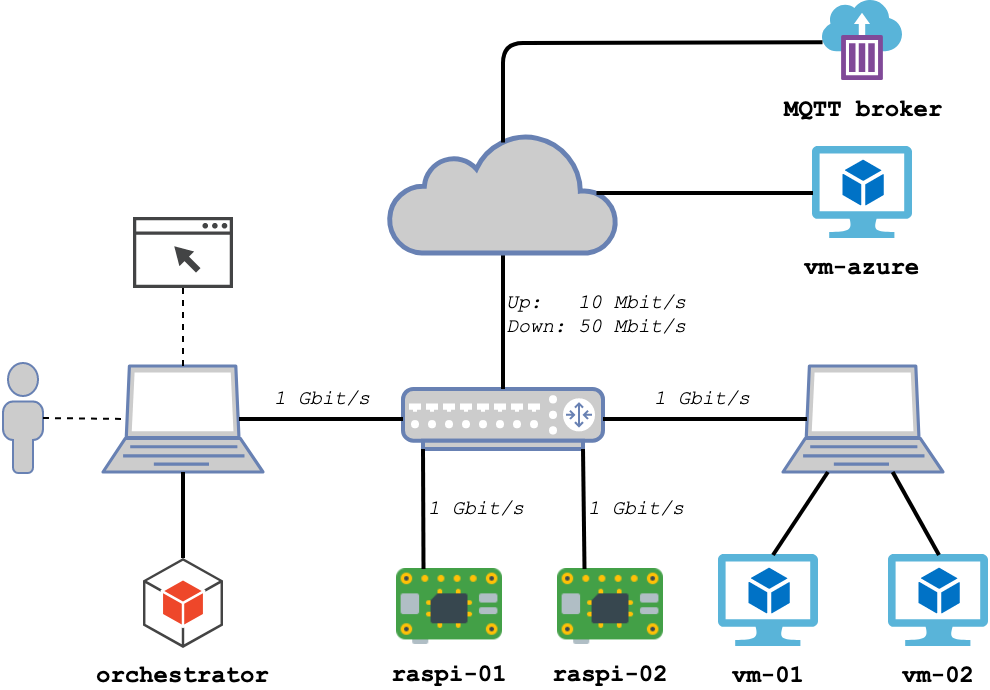
\includegraphics[width=0.85\textwidth]{evaluation-infrastructure}
    \caption{Test infrastructure for evaluation}
    \label{fig:evaluation-infrastructure}
\end{figure}

The test bed consists of the five nodes shown in figure \ref{fig:evaluation-infrastructure}. The hardware characteristics of the devices are shown in table \ref{tab:evaluation-devices}. The three virtual machines run Debian 10, the two Raspberry Pis run Raspbian 10. All nodes have \texttt{Docker version 19.03.2} installed. Another device on the local network runs the Orchestrator and a web browser which is used to access the \textit{Object Detection Web Application}. Communication between the nodes and the Orchestrator is done via an MQTT broker running in the Azure Cloud.

\begin{table}[htb]
    \centering
    \begin{tabular}{|l|l|l|l|l|l|}
    \hline
        \textbf{Node} & \textbf{Device Type} & \textbf{CPU} & \textbf{RAM} \\
         \hline
         \texttt{raspi-01} & Raspberry Pi 3B+ & ARM Cortex-A53 1.4 GHz, 4 cores & 1 GB\\
         \hline
         \texttt{raspi-02} & Raspberry Pi 4B & ARM Cortex-A72 1.5 GHz, 4 cores & 4 GB\\
         \hline
         \texttt{vm-01} & Hyper-V VM & Intel i7-8550U 1.8 GHz, 2 vCPUs & 2 GB\\
         \hline
         \texttt{vm-02} & Hyper-V VM & Intel i7-8550U 1.8 GHz, 4 vCPUs & 4 GB\\
         \hline
         \texttt{vm-azure} & Azure VM \texttt{F4s\_v2} & Intel Xeon 2.7 GHz, 4 vCPUs & 8 GB\\
         \hline
    \end{tabular}
    \caption{Hardware characteristics of test devices used for evaluation}
    \label{tab:evaluation-devices}
\end{table}

\subsection{Application\label{sec:eval-application}}

\begin{figure}[htb]
    \centering
    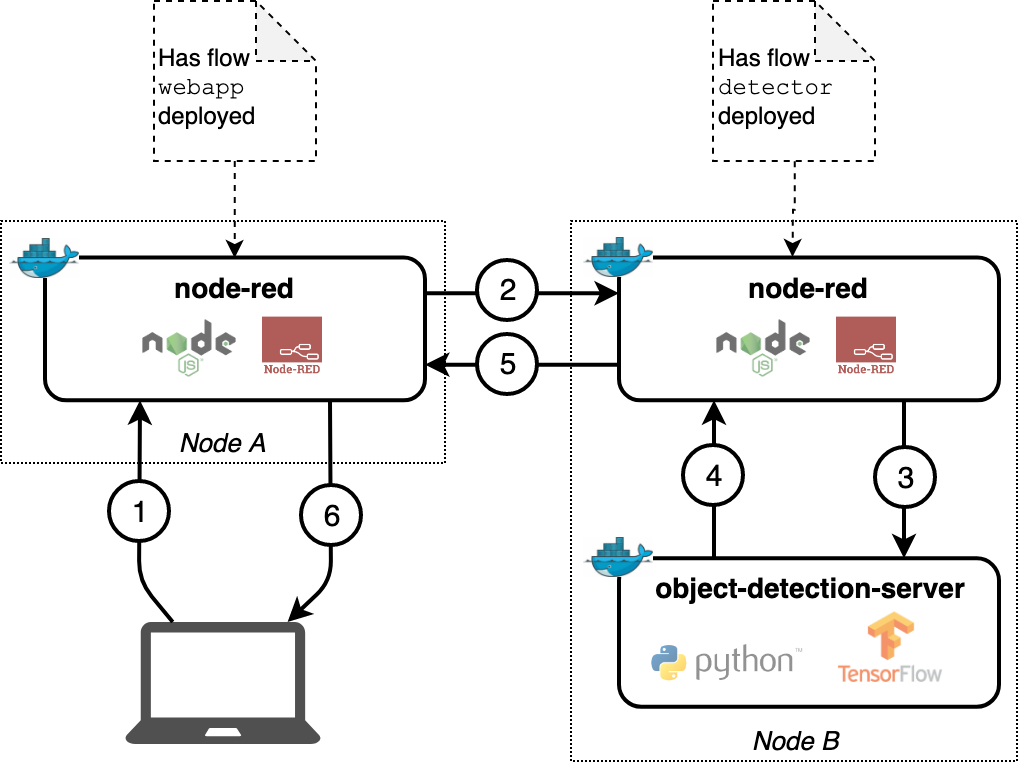
\includegraphics[width=0.85\textwidth]{evaluation-application}
    \caption{System architecture of Object Detection Web Application}
    \label{fig:evaluation-object-detection-application}
\end{figure}

The \textit{Object Detection Web Application} consists of the two modules \texttt{webapp} and \texttt{detector} as illustrated in figure \ref{fig:evaluation-object-detection-application}. A screenshot of the web application is shown in figure \ref{fig:object-detection-webapp-screenshot}.\\

In the first step, a user sends an image for object detection to the \texttt{webapp} module which is deployed as a Node-RED flow on \texttt{Node A}. This module should always be deployed on the same node and not be moved so that the web application is always available at the same address. The user calls the web application from that fixed node and he does not care which node actually executes the object detection task. The module \texttt{webapp} forwards the image to the module \texttt{detector} for object detection which is deployed on another node (\texttt{Node B}). This node can vary and is chosen by the Orchestrator. If a new node is selected by the Orchestrator, then the flow \texttt{webapp} on \texttt{Node A} will be updated so that subsequent requests are forwarded to the new node.\\

The object detection engine can not be executed as a regular Node-RED flow since Node-RED handles JavaScript functions only and the engine requires Python. Even if Node-RED could execute Python code (there are extensions enabling this) the execution of the object detection engine in Node-RED would not be efficient because the engine would have to be initialized every time a new object detection request arrives. However, the engine has a certain initialization time to load the detection graph. Therefore it is more efficient to initialize the engine only once at the beginning so that the following object detection tasks can be executed without additional initialization time. Because Node-RED can not initialize and hold Python objects, a separate docker container is used for this purpose. The flow \texttt{detector} sends an HTTP request containing the undetected image to the \texttt{object-detection-server} running on the same node. The server responds with the detected image which the \texttt{detector} then sends back to the \texttt{webapp} module.

The following three constraints are defined for the experiment:
\begin{enumerate}
    \item The flow \texttt{webapp} must be deployed on \texttt{raspi-01} because this is the only node known to the user
    \item The flow \texttt{detector} needs an \texttt{object-detection-server} docker container running on the same node which is the case for all nodes except for \texttt{raspi-01}
    \item The detected image must be available within 5 seconds
\end{enumerate}

\section{Experiment 1: Consistent network quality\label{sec:eval-exp-1}}

In this experiment, the nodes are started successively, beginning with the slowest one (regarding the total latency of the object detection application). One vCPU in \texttt{vm-01} is equally fast as in \texttt{vm-02} because they both run on the same host. Since the object detection engine uses only one core, the execution time on these two nodes is approximately the same, although \texttt{vm-01} has two cores and \texttt{vm-02} has four cores. However, for evaluating the Orchestrator we need nodes with different CPU performance(s?). For this reason, the docker containers on \texttt{vm-01} run with the additional option \texttt{---cpus="0.5"} which limits the available CPU resources a container can use to a half vCPU.

\subsection*{Possible deployment strategies and their respective latencies}
First, the application was deployed to the infrastructure without using the Orchestrator to find the real execution times of all possible deployment strategies. The module \texttt{webapp} was always deployed on node \texttt{raspi-01} while the module \texttt{detector} was switched through the remaining nodes. The object detection application was executed 10 times on each deployment strategy by using a 1.4 MB sized image. The mean values for \textit{total latency}, \textit{processing time} and \textit{transfer time} were calculated thereafter. These are compared in figure \ref{fig:evaluation-total-latency-without-orchestrator}.

\begin{figure}[h!]
    \centering
    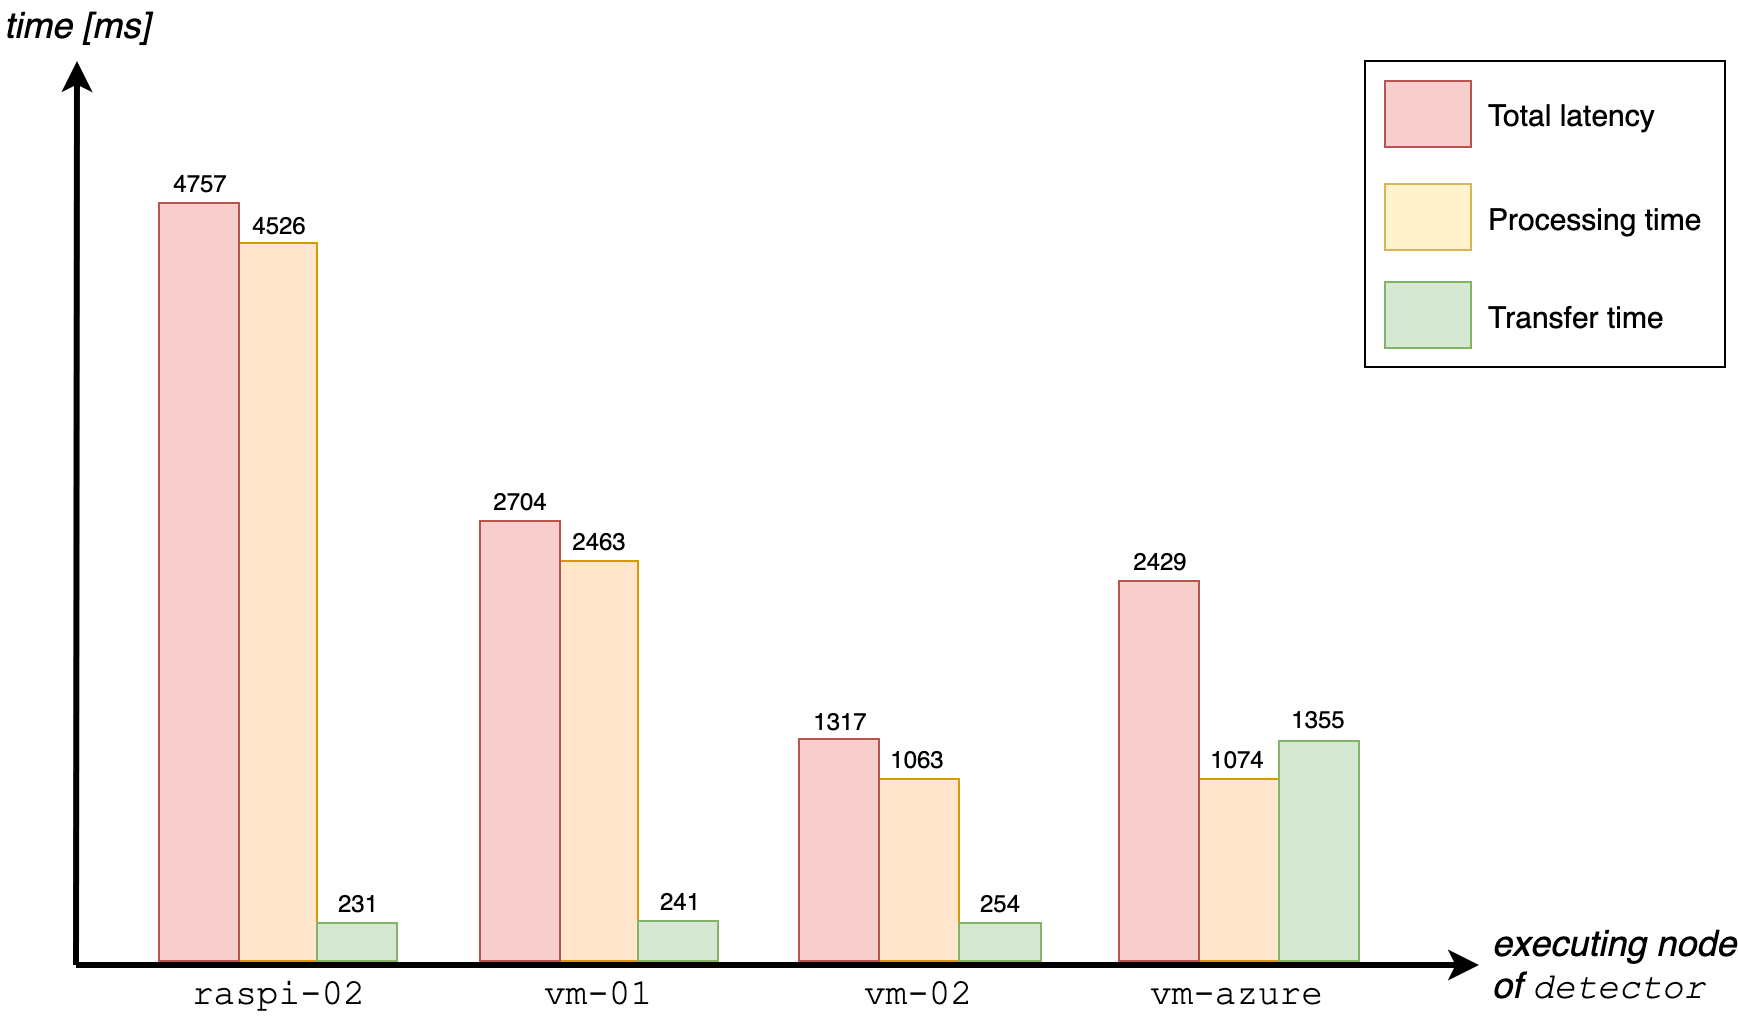
\includegraphics[width=1.0\textwidth]{evaluation-total-latency-without-orchestrator}
    \caption{Total latencies, processing and transfer times of the object detection application regarding the placement of module \texttt{detector}}
    \label{fig:evaluation-total-latency-without-orchestrator}
\end{figure}

Based on the measurement results, a prioritization of all possible deployments was created where deployments with a lower latency are preferred (see table \ref{tab:deployment-strategies-prios}).
\begin{table}[h!tb]
    \centering
    \begin{tabular}{|l|l|l|l|l|l|}
    \hline
        \textbf{Priority} & \textbf{Placement of \texttt{webapp}} & \textbf{Placement of \texttt{detector}} & \textbf{Latency} \\
         \hline
         \texttt{1} & \texttt{raspi-01} & \texttt{vm-02} & 1317 ms\\
         \hline
         \texttt{2} & \texttt{raspi-01} & \texttt{vm-azure} & 2429 ms\\
         \hline
         \texttt{3} & \texttt{raspi-01} & \texttt{vm-01} & 2704 ms\\
         \hline
         \texttt{4} & \texttt{raspi-01} & \texttt{raspi-02} & 4757 ms\\
         \hline
    \end{tabular}
    \caption{Possible deployment strategies \textcolor{red}{\textbf{for (of?)}} object detection application}
    \label{tab:deployment-strategies-prios}
\end{table}

\subsection*{Preparing the Orchestrator}

Although the Orchestrator handles the infrastructure dynamically, an application must be defined before the start of the Orchestrator. For this purpose, an instance of \texttt{Application} is created which contains all modules, loops and messages of the object detection application described in section \ref{sec:eval-application}.

\subsubsection*{Setting required RAM and storage}
The fields \texttt{requiredRam} and \texttt{requiredStorage} of the two modules \texttt{webapp} and \texttt{detector} are set to \texttt{0} because both Node-RED flows are relatively small and thus consume neither significant RAM nor storage. Although the \texttt{object-detection-server} container requires 1GB RAM, this memory is not allocated/released by deploying/removing the flow from Node-RED because the container runs even if the Node-RED flow is not deployed on the node. Furthermore, the container does not require any additional disk storage when running the engine.

\subsubsection*{Setting required hardware modules}
The field \texttt{requiredHardwareModules} of the module \texttt{webapp} contains one string: \texttt{"CAMERA"}. The \texttt{node-red} docker container on \texttt{raspi-01} is started with the additional option \texttt{-e CONNECTED\_HARDWARE=["CAMERA"]} so that \texttt{webapp} can only be deployed \textcolor{red}{\textbf{on (to?)}} \texttt{raspi-01}. The same approach is used for the module \texttt{detector}, but here the string \texttt{"OD-DOCKER-CONTAINER"} is used and passed to the docker container on the remaining nodes.

\subsubsection*{Setting required instructions}
The field \texttt{requiredMi} of the module \texttt{webapp} is set to \texttt{0} because the Node-RED flow simply forwards messages and therefore does not require any significant CPU power. However, CPU resources consumed by the module \texttt{detector} are substantial. Since the Orchestrator uses a CPU score instead of MIPS, the value for \texttt{requiredMi} has to be calculated using the formula introduced in section \ref{sec:benchmark-cpu}. Values for \textit{CPU score} and \textit{execution time} are taken from \texttt{vm-02}, which are \textit{11661} and \textit{1317 ms}, respectively. Therefore:
\[\textrm{\texttt{requiredMi\textsubscript{detector}}} = \textrm{CPU score} \boldsymbol{\cdot} \frac{\textrm{execution time [ms]}}{1000 \textrm{ [ms]}} = 11661 \boldsymbol{\cdot} \frac{1317}{1000} = 15357\]


\section{Experiment 2}

TODO

\section{Discussion}

TODO

- CPU: Intel -> gut vergleichbar; ARM -> nicht gut vergleichbar
alternative methode: test ausführung von modules und sich die zeit merken

problem: input size --> auch hier wären erfahrungswerte besser